% tikzpic.tex
\documentclass[preview,tikz]{standalone}% 'crop' is the default for v1.0, before it was 'preview'
%\usetikzlibrary{...}% tikz package already loaded by 'tikz' option
\usetikzlibrary{arrows,shapes,backgrounds}
\usepackage{ifthen}
\begin{document}
\tikzstyle{background grid}=[draw, blue!30,step=.5cm,very thin]
	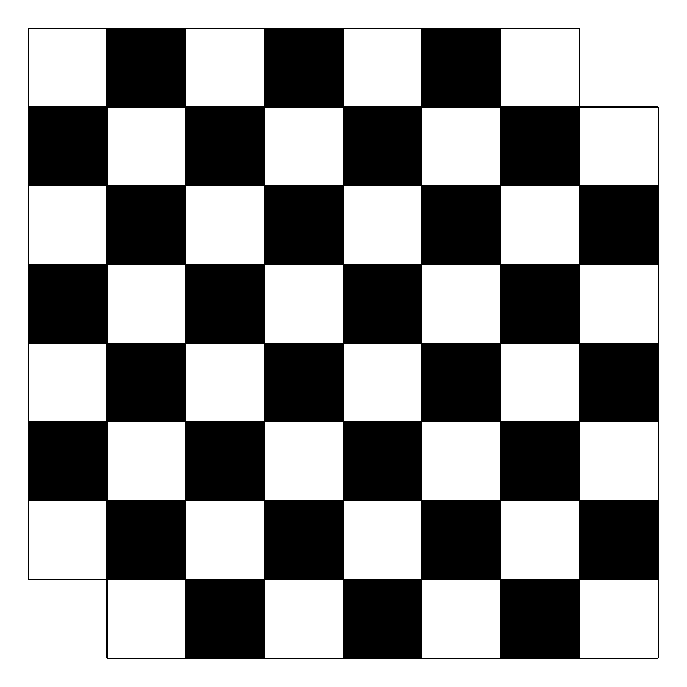
\begin{tikzpicture}[x=1cm]
%	\foreach \y in {2,4,...,6}{
%		\foreach \x in {0,2,...,6}{
%			\draw[fill=black] (\x,\y) rectangle (1+\x,1+\y) rectangle (2+\x,2+\y);
%			\draw[] (\x, 2+\y) rectangle (\x+1, \y+1) rectangle (2+\x, \y);
%		}
%	}
	\foreach \x in {1,2,3,4,5,6}{
		\draw (\x, 0) -- (\x, 8);
	}
	\draw(0, 1) -- (0,8);
	\draw(8,0) -- (8,7);
	\draw(1,0) -- (8,0);
	\draw(0,8) -- (7,8);
	\draw(7,8) -- (7,7) -- (8,7);
	\foreach \y in {1,2,3,4,5,6}{
		\draw (0, \y) -- (8, \y);
	}
	
\draw[fill=black] (0,2) rectangle (1,3);
\draw[fill=black] (0,4) rectangle (1,5);
\draw[fill=black] (0,6) rectangle (1,7);
\draw[fill=black] (1,1) rectangle (2,2);
\draw[fill=black] (1,3) rectangle (2,4);
\draw[fill=black] (1,5) rectangle (2,6);
\draw[fill=black] (1,7) rectangle (2,8);
\draw[fill=black] (2,0) rectangle (3,1);
\draw[fill=black] (2,2) rectangle (3,3);
\draw[fill=black] (2,4) rectangle (3,5);
\draw[fill=black] (2,6) rectangle (3,7);
\draw[fill=black] (3,1) rectangle (4,2);
\draw[fill=black] (3,3) rectangle (4,4);
\draw[fill=black] (3,5) rectangle (4,6);
\draw[fill=black] (3,7) rectangle (4,8);
\draw[fill=black] (4,0) rectangle (5,1);
\draw[fill=black] (4,2) rectangle (5,3);
\draw[fill=black] (4,4) rectangle (5,5);
\draw[fill=black] (4,6) rectangle (5,7);
\draw[fill=black] (5,1) rectangle (6,2);
\draw[fill=black] (5,3) rectangle (6,4);
\draw[fill=black] (5,5) rectangle (6,6);
\draw[fill=black] (5,7) rectangle (6,8);
\draw[fill=black] (6,0) rectangle (7,1);
\draw[fill=black] (6,2) rectangle (7,3);
\draw[fill=black] (6,4) rectangle (7,5);
\draw[fill=black] (6,6) rectangle (7,7);
\draw[fill=black] (7,1) rectangle (8,2);
\draw[fill=black] (7,3) rectangle (8,4);
\draw[fill=black] (7,5) rectangle (8,6);
	
%	\foreach \x in {0,1,...,7}{
%		\node() at (\x+0.5, -0.5) {\x};
%	}
%	\node() at (4,-1){x};
%	\foreach \x in {0,1,...,7}{
%		\node() at (-0.5, \x+0.5) {\x};
%	}
%	\node() at (-1,4){y};		
%	\node[anchor=center, red] at (5.5,5.5) {\huge{B}};
%	\draw[very thick, red, ->] (5,5) -- (3,3);
%	\draw[very thick, red,->] (6,6) -- (8,8);	
%	\draw[very thick, red,->] (5,6) -- (3,8);
%	\draw[very thick, red,->] (6,5) -- (8,3);
	\end{tikzpicture}
\end{document}
